\tikzstyle{s} = [rectangle, rounded corners, minimum width=2cm, text width=2cm, minimum height=1cm, text centered, draw=black]
\tikzstyle{arrow} = [thick,->,>=stealth]
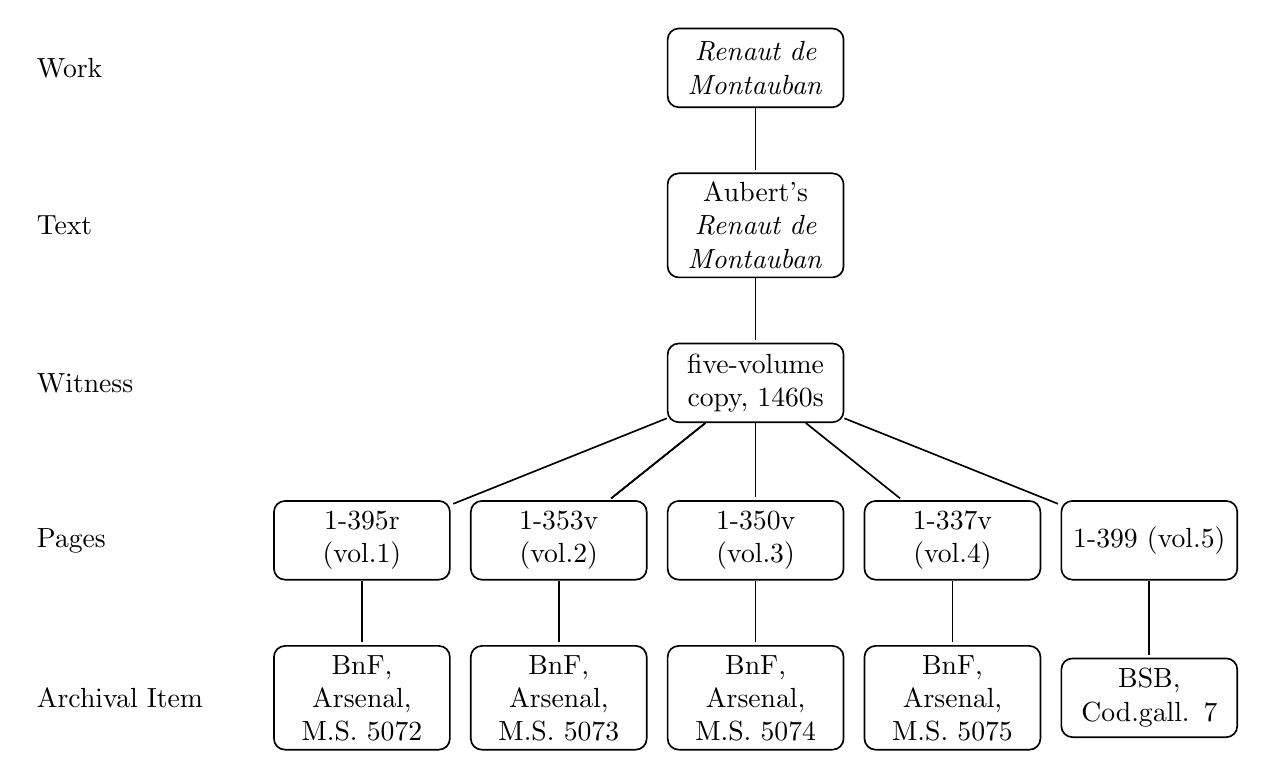
\begin{tikzpicture}[-,shorten >=1pt,auto,node distance=2cm,semithick]
\tikzstyle{every state}=[fill=red,draw=none,text=white]

\node[s] (Wk) {\textit{Renaut de Montauban}};
\node [left=6cm, text width=3cm] at (Wk) {Work};

\node[s] (T) [below of=Wk] {Aubert's \textit{Renaut de Montauban}};
\node [left=6cm, text width=3cm] at (T) {Text};

\node[s] (W) [below of=T] {five-volume copy, 1460s};
\node [left=6cm, text width=3cm] at (W) {Witness};

\node[s] (V3) [below of=W] {1-350v (vol.3)};
\node[s] (V2) [left of=V3, xshift=-0.5cm] {1-353v (vol.2)};
\node[s] (V1) [left of=V2, xshift=-0.5cm] {1-395r (vol.1)};
\node[s] (V4) [right of=V3, xshift=0.5cm] {1-337v (vol.4)};
\node[s] (V5) [right of=V4, xshift=0.5cm] {1-399 (vol.5)};
\node [left=1cm, text width=3cm] at (V1) {Pages};

\node[s] (D1) [below of=V1] {BnF, Arsenal, M.S. 5072};
\node[s] (D2) [below of=V2] {BnF, Arsenal, M.S. 5073};
\node[s] (D3) [below of=V3] {BnF, Arsenal, M.S. 5074};
\node[s] (D4) [below of=V4] {BnF, Arsenal, M.S. 5075};
\node[s] (D5) [below of=V5] {BSB, Cod.gall. 7};
\node [left=1cm, text width=3cm] at (D1) {Archival Item};

\path[every node/.style={font=\sffamily\small}]
    (Wk) edge node [right] {} (T)
    (T) edge node [right] {} (W)
    (W) edge node [right] {} (V1)
    (W) edge node [right] {} (V2)
    (W) edge node [right] {} (V2)
    (W) edge node [right] {} (V3)
    (W) edge node [right] {} (V4)
    (W) edge node [right] {} (V5)
    (V1) edge node [right] {} (D1)
    (V2) edge node [right] {} (D2)
    (V3) edge node [right] {} (D3)
    (V4) edge node [right] {} (D4)
    (V5) edge node [right] {} (D5)
    ;

\end{tikzpicture}